\documentclass{beamer}
\usetheme[titleformat=regular,sectiontitleformat=regular,frametitleformat=regular]{m}

\usepackage[brazil]{babel}
\usepackage[numberedbib]{apacite}
\usepackage[utf8]{inputenc}
\usepackage{mathabx}

\title{Apresentação de artigo: A Genetic Programming Approach to Record Deduplication}
\date{\today}
\author{Herberth Amaral}
\institute{Programa de Pós-Graduação em Modelagem Computacional e Sistemas - UNIMONTES}
\begin{document}
  \maketitle

  \section{Introdução}

  \begin{frame}{Record linkage}
      \textit{Record linkage} (RL) é o processo de encontrar registros duplicados que representam a mesma entidade em um ou mais conjuntos de dados \cite{survey}.

      Faz parte das tarefas de \textit{data cleaning} dos processos de mineração de dados.
  \end{frame}

  \section{Teoria de RL}

  \begin{frame}{Modelagem matemática}
      Modelo desenvolvido por \cite{fellegi69}. Foi a primeira tentativa bem sucedida de criar um modelo matemático para RL.

      Compreende três decisões: \textit{link} ($A_1$), \textit{non-link} ($A_3$) e \textit{potential link} ($A_2$). 

  \end{frame}

  \begin{frame}{Modelagem matemática}
      Considere dois \textit{datasets}, $A$ e $B$. Vamos assumir que alguns elementos são comuns entre $A$ e $B$. Consequentemente a união dos dois conjuntos disjuntos é:
      \begin{center}
          $A \bigtimes B = \{(a,b); a \in A, b \in B\}$
      \end{center}
      E os conjuntos que chamamos de \textit{matched} e \textit{unmatched} são respectivamente:
      \begin{center}
          $M = \{(a,b); a=b, a \in A, b \in B\}$ \\
          $U = \{(a,b); a \neq b, a \in A, b \in B\}$
      \end{center}

  \end{frame}
  \begin{frame}{Modelagem matemática}
      Para o processo de record linkage, cada par de tuplas $(a,b)$ precisa ser comparado atributo-por-atributo. Então, o \textit{vetor de comparações} dos registros $\alpha(a), \beta(b)$ pode ser definido como:
      \begin{center}
          $\gamma[\alpha(a),\beta(b)] = \{\gamma^1[\alpha(a), \beta(b)],\cdots, \gamma^k[\alpha(a), \beta(b)]\}$
      \end{center}
      $\gamma$ é uma função em $A \bigtimes B$ e o conjunto de todos os possíveis $\gamma(\alpha(a),\beta(b))$ compõe o espaço de busca $\Gamma$.
  \end{frame}

  \begin{frame}{Modelagem matemática}
      Para sabermos se $(a,b)$ realmente são a mesma entidade (ou seja, $(a,b) \in M$), precisamos definir uma \textit{regra de ligação} que mapeia $\Gamma$ em um conjunto aleatório de funções de decisão $D = \{d(\gamma)\}$ em que
      \begin{center}
          $d(\gamma) = \{P(A_1|\gamma), P(A_2|\gamma), P(A_3|\gamma)\}; \gamma \in \Gamma$ \\
          $\sum\limits_{i=1}^3 P(A_i|\gamma) = 1$
      \end{center}
      Ou seja, para cada valor observado de $\gamma$, a regra de ligação associa as possibilidades de \textit{link} ($A_1$), \textit{potential link} ($A_2$) e \textit{non-link} ($A_3$).
  \end{frame}

  \begin{frame}{Modelagem matemática}
      Uma regra de ligação ótima minimiza $P(A_2|\gamma) \forall \gamma \in \Gamma$. Dependendo dos datasets A e B, a regra de ligação ótima pode ser difícil de se obter. Sendo a regra de ligação uma \textbf{função}, podemos \textbf{evolui-la} através de um processo conhecido como \textbf{programação genética}.
  \end{frame}

  \begin{frame}{Programação genética}
      Programação evolucionária é baseada em idéias inspiradas do processo que influencia virtualmente todos os seres vivos, a \textit{seleção natural} \cite{geneticrl}.

      Programação gentética (GP) é uma das técnicas mais conhecidas dentro da programação evolucionária. Pode ser visto como uma heurística adaptativa em que as idéias básicas vem das propriedades das operações genéticas e seleção natural.

      A principal diferença entre GP e outras técnicas evolucionárias é que GPs representam o conceito do problema como um programa de computador. Ou seja, cada indivíduo é uma \textbf{\textit{função}}, representado como uma \textbf{\textit{árvore}}.
  \end{frame}
  \begin{frame}{Programação genética - algoritmo básico}
      \begin{enumerate}
          \item Inicialize a população;
          \item Avalia todos os indivíduos, associando uma nota (\textit{fitness}) a cada um;
          \item Execute o último passo se o critério de parada for atingido. Do contrário, continue;
          \item \textbf{Selecione} os melhores $n$ indivíduos para a próxima geração;
          \item Aplique os operadores de \textbf{cruzamento} e \textbf{mutação} para obter $m$ novos indivíduos;
          \item Substitua a população atual pela população gerada ao passo 2;
          \item Apresente o melhor indivíduo na população como saída do processo evolucionário.
      \end{enumerate}
  \end{frame}
  \begin{frame}{Programação genética - Operadores}
      Programação genética, assim como demais algoritmos evolucionários, possuem métodos para representar o procsso evolutivo:
      \begin{enumerate}
          \item Seleção;
          \item Cruzamento;
          \item Mutação;
      \end{enumerate}
  \end{frame}

  \begin{frame}{Programação genética - Seleção}
      É a operação que copia os indivíduos sem os modificar. Geralmente é feito com uma estratégia elitista, que mantém os melhores indivíduos para a próxima geração.
  \end{frame}

  \begin{frame}{Programação genética - Cruzamento}
      Permite que material genético (ou seja, sub-árvores) seja trocado entre dois pais em um processo que pode gerar um ou mais filhos. Os filhos são o resultado da troca das sub-árvores selecionadas entre os pais, conforme ilustrado na figura \ref{fig:crossover}.
      \begin{figure}
          \centering
          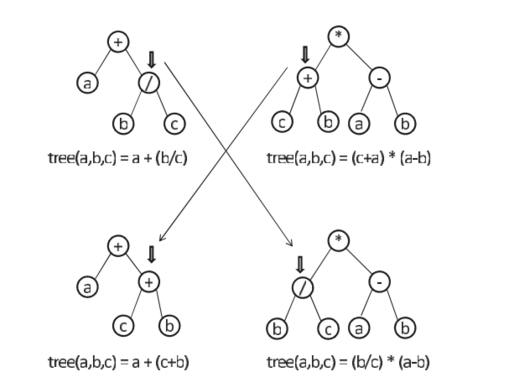
\includegraphics[width=0.4\textwidth]{crossover.png}
          \caption{Cruzamento entre árvores \cite{geneticrl}}
          \label{fig:crossover}
      \end{figure}
  \end{frame}

  \begin{frame}{Programação genética - Cruzamento}
      Permite que material genético (ou seja, sub-árvores) seja trocado entre dois pais em um processo que pode gerar um ou mais filhos. Os filhos são o resultado da troca das sub-árvores selecionadas entre os pais, conforme ilustrado na figura \ref{fig:crossover}.
      \begin{figure}
          \centering
          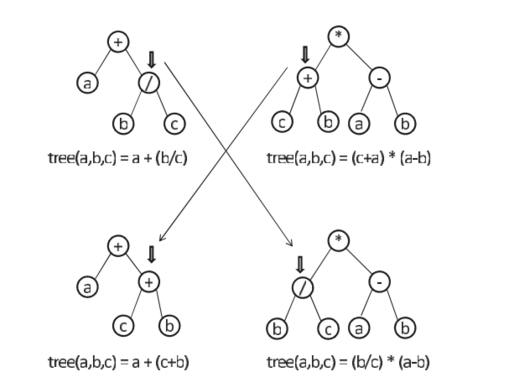
\includegraphics[width=0.4\textwidth]{crossover.png}
          \caption{Cruzamento entre árvores \cite{geneticrl}}
          \label{fig:crossover}
      \end{figure}
  \end{frame}

  \begin{frame}{Programação genética - Mutação}
      O operador de mutação possui o papel de aumentar a diversidade e, assim, fazer com que o PG explore melhor seu espaço de busca. Todos os indivíduos tem uma chance fixa de sofrer mutação. Numa árvore GP, um nó aleatório é selecionado e a sub-árvore correspondente é trocada por uma aleatoriamente criada, conforme ilustrado na figura \ref{fig:mutacao}.
      \begin{figure}
          \centering
          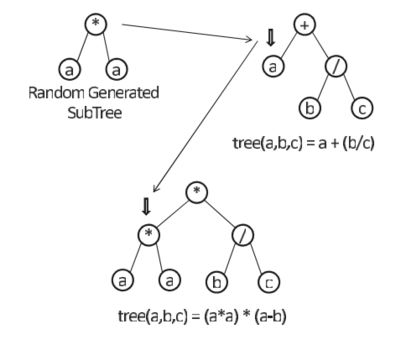
\includegraphics[width=0.4\textwidth]{mutacao.png}
          \caption{Mutação de sub-árvore \cite{geneticrl}}
          \label{fig:mutacao}
      \end{figure}
  \end{frame}

  \section{Modelando o problema de record linkage com programação genética}

  \begin{frame}{Modelagem de RL com GP}
      A função que os autores evoluem tomam como parâmetro um conjunto de \textit{evidências}, em que cada evidência $E$ é um par $<atributo, func. similaridade>$. 

      Por exemplo, suponha que queiramos deduplicar uma base em que cada instância tenha os atributos nome, sobrenome e endereço. Usando uma função de similaridade (ex. Jaro), podemos ter a seguinte lista de similaridades: $(E_1<nome, Jaro>, E_2<sobrenome, Jaro>, E_3<endereco, Jaro>)$.

      Uma função de similaridade simples seria a combinação linear das evidências, como por exemplo $F_s(E_1, E_2, E_3) = E_1+E_2+E_3$.
  \end{frame}

  \begin{frame}{Modelagem de RL com GP}
      Na modelagem cada evidência é colocada numa folha da árvore. Cada folha pode também ser um número real aleatório entre 1.0 e 9.0, que é escolhido quando a árvore é gerada.

      A saída da função é um valor numérico que servirá para dizer se os registros representados pelas evidências são os mesmos ou não. Para isso é adotado um limiar e todas os pares cujo os valores são acima desse limiar são consideradas como um \textit{match}.

      A função de \textit{fitness} utilizada na evolução da árvore é o F1-score, que combina duas métricas bem utilizadas: revocação (\textit{recall}) e precisão e é definida da seguinte forma:

      \begin{center}
          $P = \frac{NumeroDeDuplicatasCorretamenteIdentificadas}{NumeroDeParesIdentificados}$ \\
          $R = \frac{NumeroDeDuplicatasCorretamenteIdentificadas}{NumeroVerdadeiroDeParesDuplicados}$ \\
          $F1 = \frac{2PR}{P+R}$ \\
      \end{center}
  \end{frame}

  \section{Experimentos}

  \begin{frame}{Experimentos}
      \begin{enumerate}
          \item O GP foi usado para encontrar a melhor combinação das evidências, com evidências manualmente selecionadas. Essa estratégia é comum em outros trabalhos relacionados.
          \item O GP foi usado para encontrar a melhor combinação das evidências, com evidências automaticamente selecionadas
      \end{enumerate}

      Os datasets utilizados foram:
      \begin{enumerate}
          \item \textbf{Cora bibliographic} - uma coleção de citações - 1295 instâncias. \textbf{Atributos}: \textit{author names, year, title, venue, pages} e \textit{other info}.
          \item \textbf{Restaurant dataset} - endereços de restaurantes -- 864 instâncias, sendo 112 duplicadas. \textbf{Atributos}: \textit{name, address, city} e \textit{specialty}.
          \item Datasets genéricos utilizando o SDG do FEBRL.
      \end{enumerate}
  \end{frame}

  \begin{frame}{Experimentos - Configuração do GP}

      \begin{figure}
          \centering
          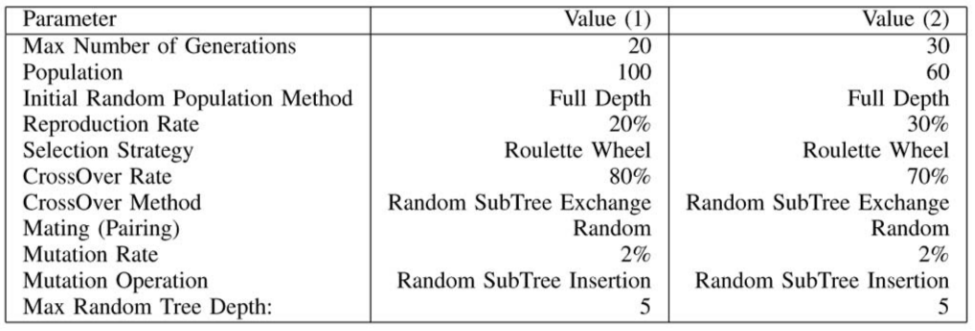
\includegraphics[width=0.75\textwidth]{parametrosga.png}
          \caption{Parâmetros do GP\cite{geneticrl}}
          \label{fig:param}
      \end{figure}
  \end{frame}

  \begin{frame}{Experimentos - evidência manualmente selecionadas}
      A imagen \ref{fig:tbl1} mostram os resultados dos testes executados.
      \begin{figure}
          \centering
          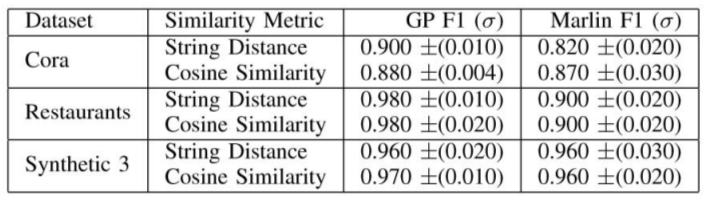
\includegraphics[width=0.75\textwidth]{resultados-manuais.png}
          \caption{Resultados da estratégia manual \cite{geneticrl}}
          \label{fig:tbl1}
      \end{figure}
  \end{frame}

  \begin{frame}{Experimentos - evidências automaticamente selecionadas}
      \begin{figure}
          \centering
          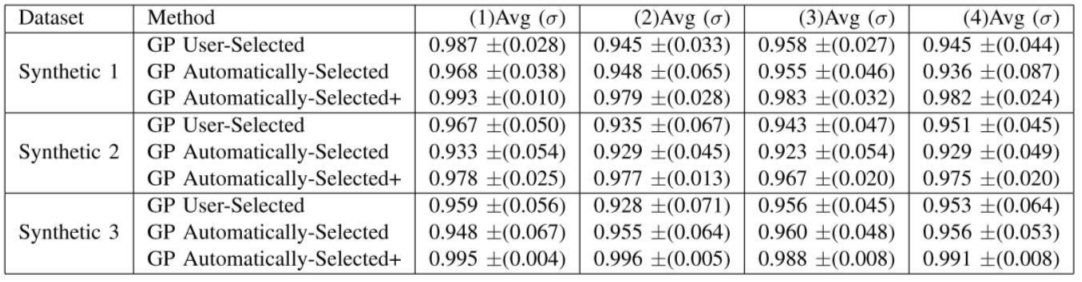
\includegraphics[width=0.9\textwidth]{resultados-automaticos.png}
          \caption{Resultados com evidências automaticamente selecionadas \cite{geneticrl}}
          \label{fig:resultados-automaticos}
      \end{figure}
  \end{frame}

  \begin{frame}{Experimentos - tempos de treinamento e validação para o dataset sintético}
      \begin{figure}
          \centering
          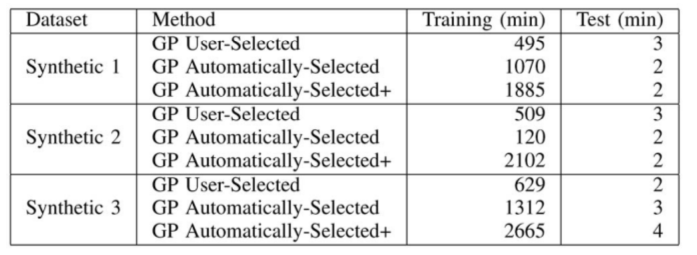
\includegraphics[width=0.9\textwidth]{tempos.png}
          \caption{Tempos de treinamento e validação para o dataset sintético \cite{geneticrl}}
          \label{fig:tempos}
      \end{figure}
  \end{frame}


  \section{Referências}
      \begin{frame}{Referências}
          \bibliographystyle{apacite}
          \bibliography{apresentacao}
      \end{frame}
\end{document}
